\documentclass[border=4pt]{standalone}
\usepackage{pgfplots}
\usepgfplotslibrary{fillbetween}
\pgfplotsset{compat=1.18}

\begin{document}
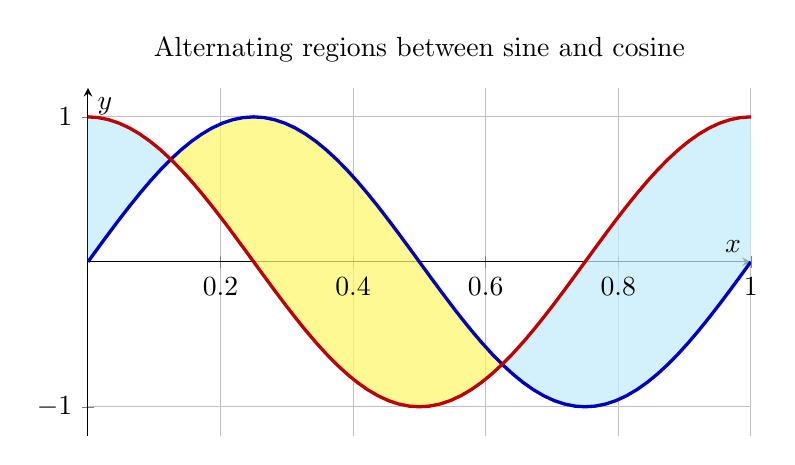
\begin{tikzpicture}
  \begin{axis}[
    width=10cm,
    height=6cm,
    xmin=0,
    xmax=1,
    ymin=-1.2,
    ymax=1.2,
    axis lines=middle,
    grid=major,
    xlabel={$x$},
    ylabel={$y$},
    title={Alternating regions between sine and cosine}
  ]
    \addplot[
      name path=sinpath,
      blue!75!black,
      very thick,
      domain=0:1,
      samples=65
    ] {sin(360*x)};
    \addplot[
      name path=cospath,
      red!75!black,
      very thick,
      domain=0:1,
      samples=65
    ] {cos(360*x)};
    \addplot[fill=cyan!24,fill opacity=0.72] fill between[
      of=sinpath and cospath,
      split,
      every even segment/.style={fill=cyan!24},
      every odd segment/.style={fill=yellow!58}
    ];
  \end{axis}
\end{tikzpicture}
\end{document}
